\documentclass[conference]{IEEEtran}
\IEEEoverridecommandlockouts
% The preceding line is only needed to identify funding in the first footnote. If that is unneeded, please comment it out.
\usepackage{cite}
\usepackage{amsmath,amssymb,amsfonts}
\usepackage{algorithmic}
\usepackage{graphicx}
\usepackage{textcomp}
\usepackage{xcolor}
\usepackage{booktabs}
\usepackage{hyperref}

\def\BibTeX{{\rm B\kern-.05em{\sc i\kern-.025em b}\kern-.08em
    T\kern-.1667em\lower.7ex\hbox{E}\kern-.125emX}}

\begin{document}

\title{Predicting Patient No-Shows to Optimize Infusion Center Scheduling}

\author{\IEEEauthorblockN{Pierce Daugherty}
\IEEEauthorblockA{\textit{School of Computer Science} \\
\textit{CS 451: Data Science Final Project}\\
Spring 2026}
}

\maketitle

\begin{abstract}
Patient no-shows in outpatient infusion centers cause severe operational inefficiencies, including wasted clinical staff time and delayed care for other patients. Predicting no-shows allows healthcare providers to implement targeted reminders and optimize scheduling capacities. This work develops an end-to-end machine learning pipeline to predict appointment no-shows using a historical dataset of over 110,000 medical appointments. Through data cleaning and feature engineering - such as deriving lead times, identifying prior no-show rates, and categorizing appointment days - we trained and evaluated Logistic Regression, Random Forest, and Gradient Boosting models. Our top-performing Random Forest model identified high-risk appointments with improved precision and recall, optimized via GridSearchCV and evaluated using Precision, Recall, F1-score, and ROC-AUC. Results suggest that behavioral history and appointment lead time are heavy drivers of attendance. We outline our findings and describe how models were operationalized into a Streamlit application, allowing scheduling teams to perform dynamic re-allocation, enabling improved scheduling decisions that may reduce idle capacity and improve patient access.
\end{abstract}

\begin{IEEEkeywords}
no-show prediction, machine learning, healthcare operations, predictive modeling
\end{IEEEkeywords}

\section{Introduction}
Missed appointments, commonly known as ``no-shows,'' are a pervasive challenge in healthcare. For specialized outpatient infusion centers, such as IVX Health, these missed appointments create significant logistical and financial strain. Infusion therapies often require expensive medications, dedicated nursing staff, and specialized infusion chairs. When a patient fails to show up, the center incurs non-recoverable staffing costs and misses an opportunity to treat patients waiting for critical care.

Optimizing scheduling directly impacts center profitability, capacity for strategic growth, and overall patient satisfaction. The overarching objective of this work is to build an effective predictive model for determining the likelihood of a patient missing an infusion appointment. By identifying high-risk appointments, clinical scheduling teams can leverage targeted interventions, such as personalized follow-up calls or intelligent double-booking, to mitigate the impact of no-shows. 

In this work, we present an end-to-end data pipeline originating from raw patient scheduling records to deployed insights. We investigate the relationship between a patient's behavioral history, demographic features, appointment lead times, and the likelihood of attendance. Finally, we formulate a scheduling dashboard via Streamlit to turn predictive probabilities into actionable scheduling decisions.

\section{Related Work}
The prediction of patient no-shows has been heavily studied in healthcare operations management. Early works predominantly focused on descriptive statistics to identify high-risk populations. With the advent of machine learning, numerous studies have applied predictive analytics to clinic schedules.

Dantas et al. \cite{dantas2018predicting} explored predicting appointment no-shows utilizing classification models ranging from simple logistical regressions to advanced decision trees. Their findings emphasize that prior patient attendance history is heavily correlated with future behavior. Similarly, Samorani et al. \cite{samorani2020overbooking} studied how predicting no-shows can directly fuel intelligent overbooking policies, minimizing the cost of wasted physician time. Other foundational research, such as works by Alaeddini et al. \cite{alaeddini2011predicting} and Huang et al. \cite{huang2014patient}, demonstrates that augmenting electronic health records with socio-demographic features can further enhance model discrimination.

Our project is partly inspired by the popular ``Medical Appointment No Shows'' Kaggle competition \cite{hoppen2016medical}. We extend the general strategies derived from Kaggle by rigorously incorporating synthetic operational elements suited for a modern infusion center workflow, deploying these insights actively into a dashboard for immediate administrative use \cite{streamlit}.

\section{Data Description}
The primary dataset utilized is a publicly available Brazilian medical appointment recordset spanning over 110,000 observations \cite{hoppen2016medical}. 

\subsection{Basic Characteristics}
The uncleaned dataset contains 110,527 records with 14 features, capturing attributes such as patient demographics, appointment scheduling dates, receipt of SMS reminders, and diagnoses for chronic conditions (e.g., Hypertension, Diabetes). The target variable, \texttt{No-show}, is originally encoded as strict binary strings. 

\subsection{Exploratory Data Analysis}
Through exploratory data analysis (EDA), we uncovered key distributions. A counterintuitive observation was the relationship between SMS reminders and no-shows (see Fig. \ref{fig:sms}). SMS reminders were seemingly correlated with high no-show rates; however, this is likely attributed to a selection bias where SMS reminders were disproportionately dispatched to historically high-risk patients. 

\begin{figure}[htbp]
\centerline{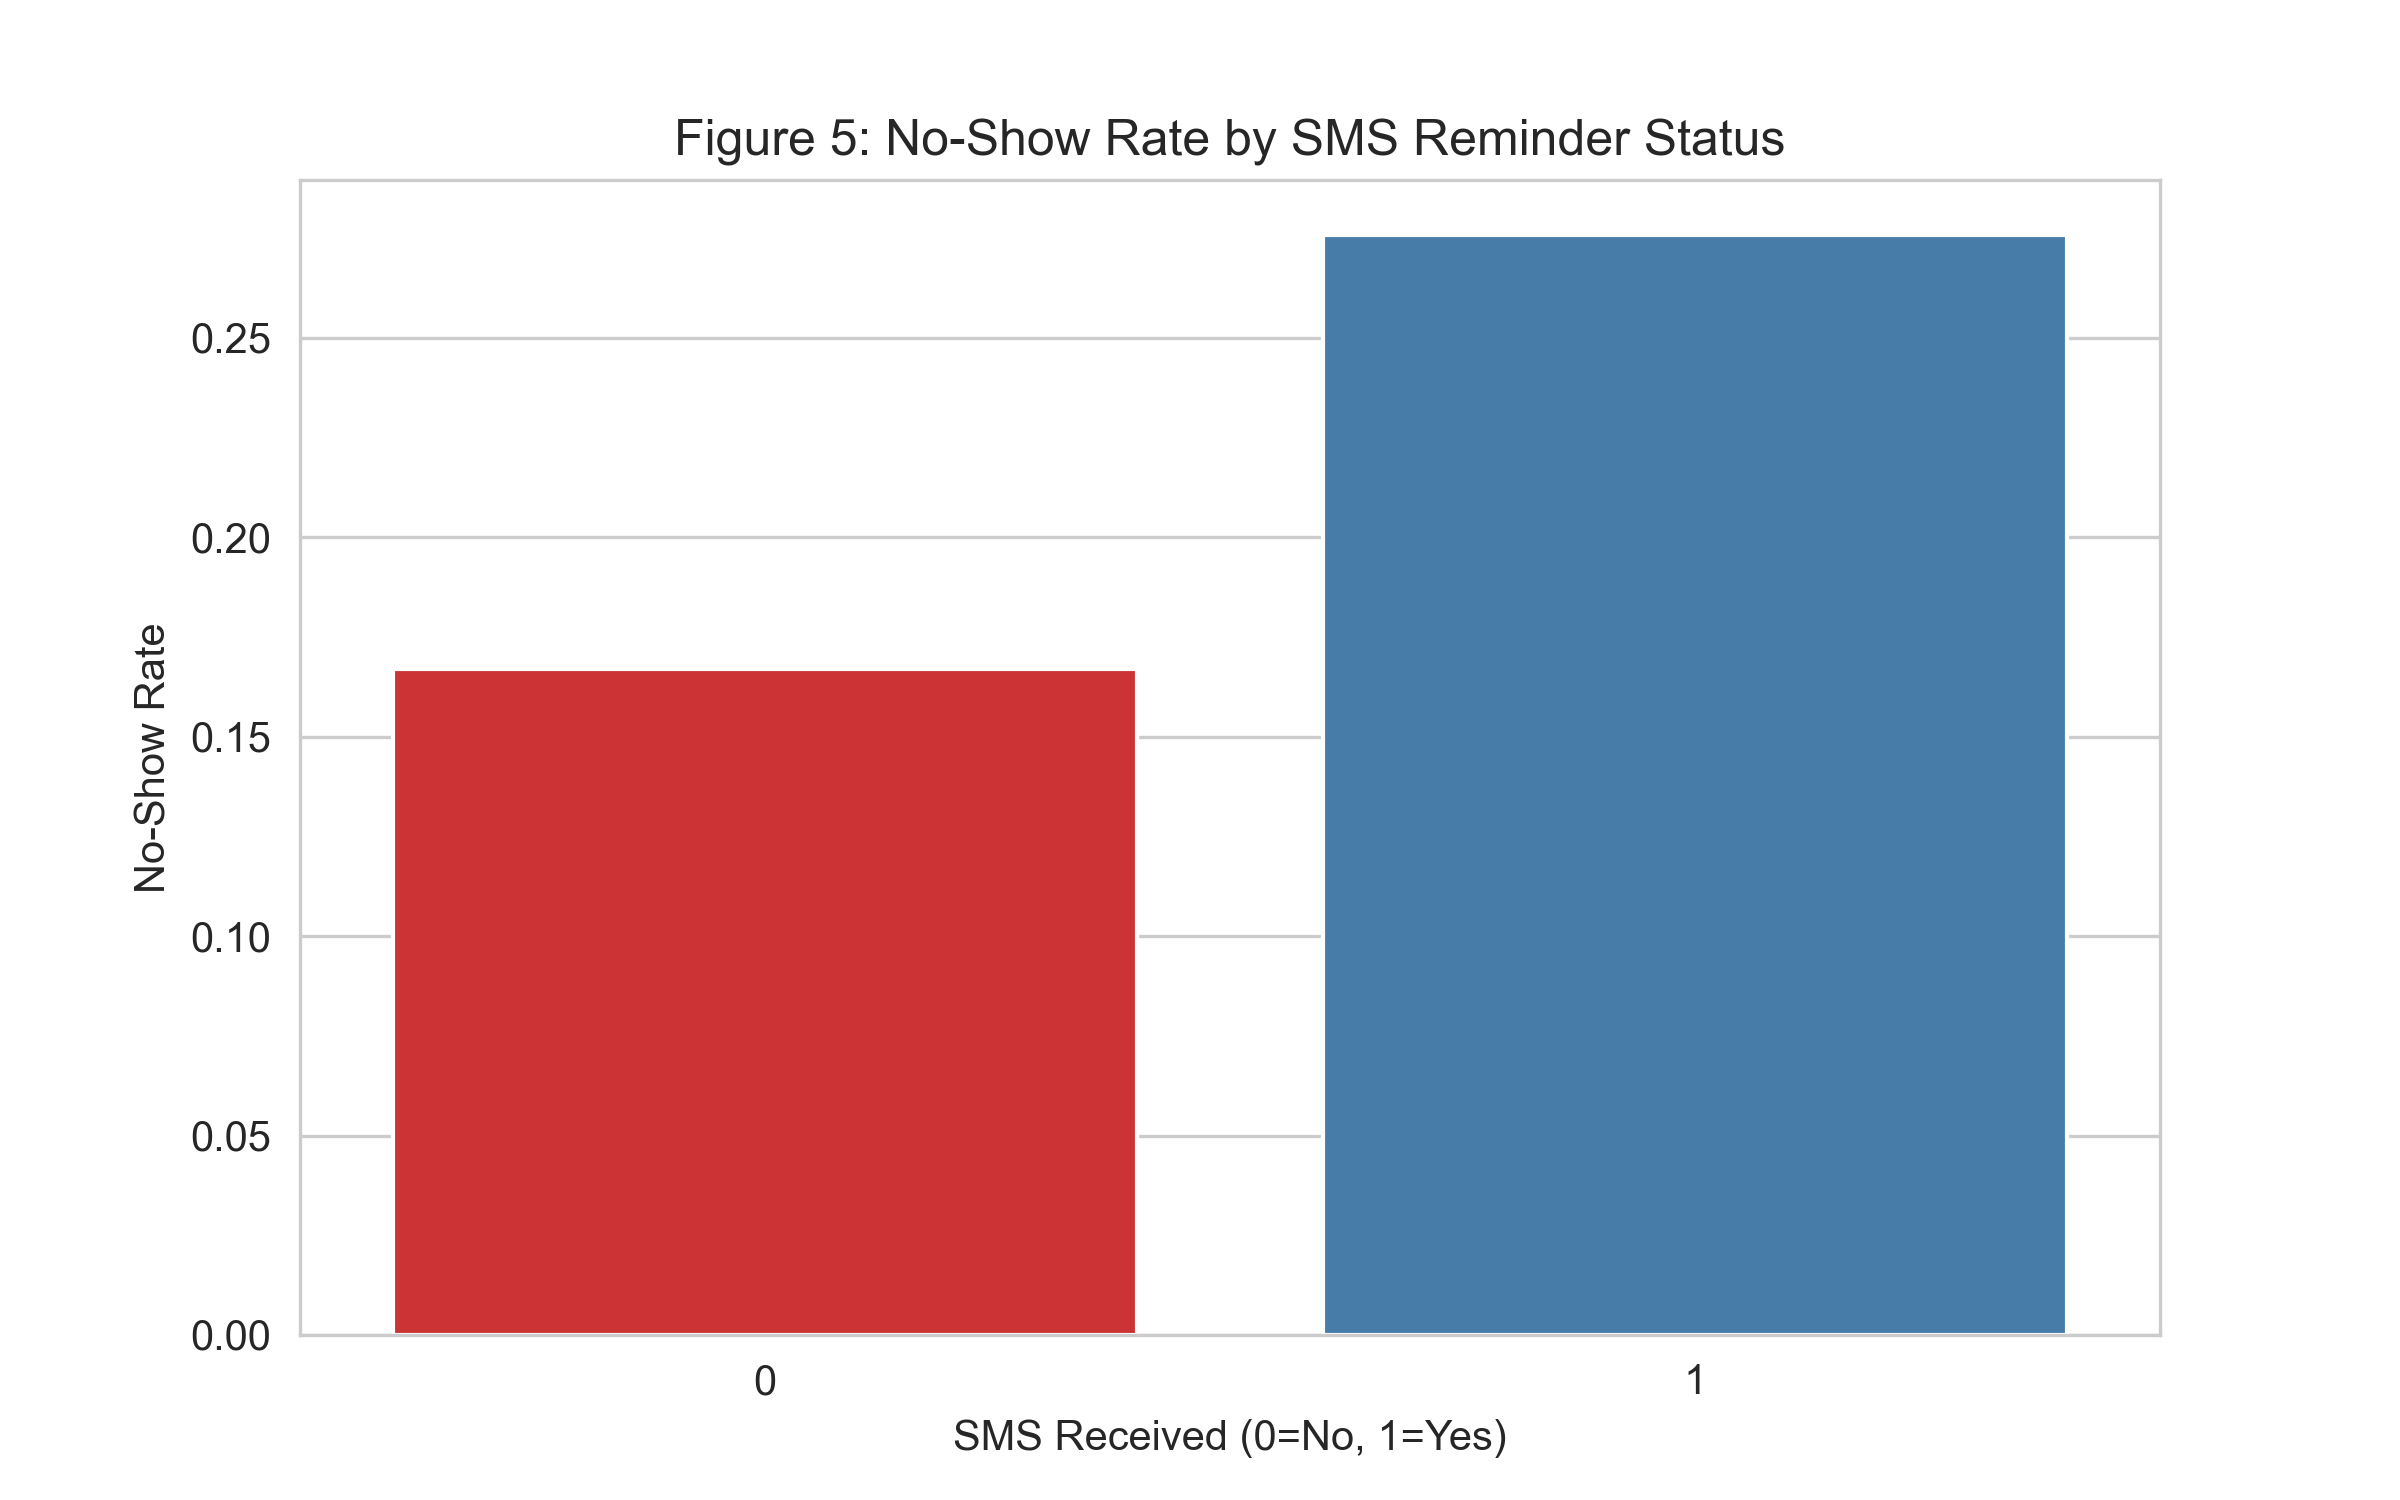
\includegraphics[width=\columnwidth]{figures/fig5_sms_effect.png}}
\caption{Effect of SMS reminders on no-show rates, illustrating selection bias.}
\label{fig:sms}
\end{figure}

Data also confirmed that lengthy \textit{lead times} between the scheduling date and the appointment date heavily degraded patient attendance (see Fig. \ref{fig:lead_time}).

\begin{figure}[htbp]
\centerline{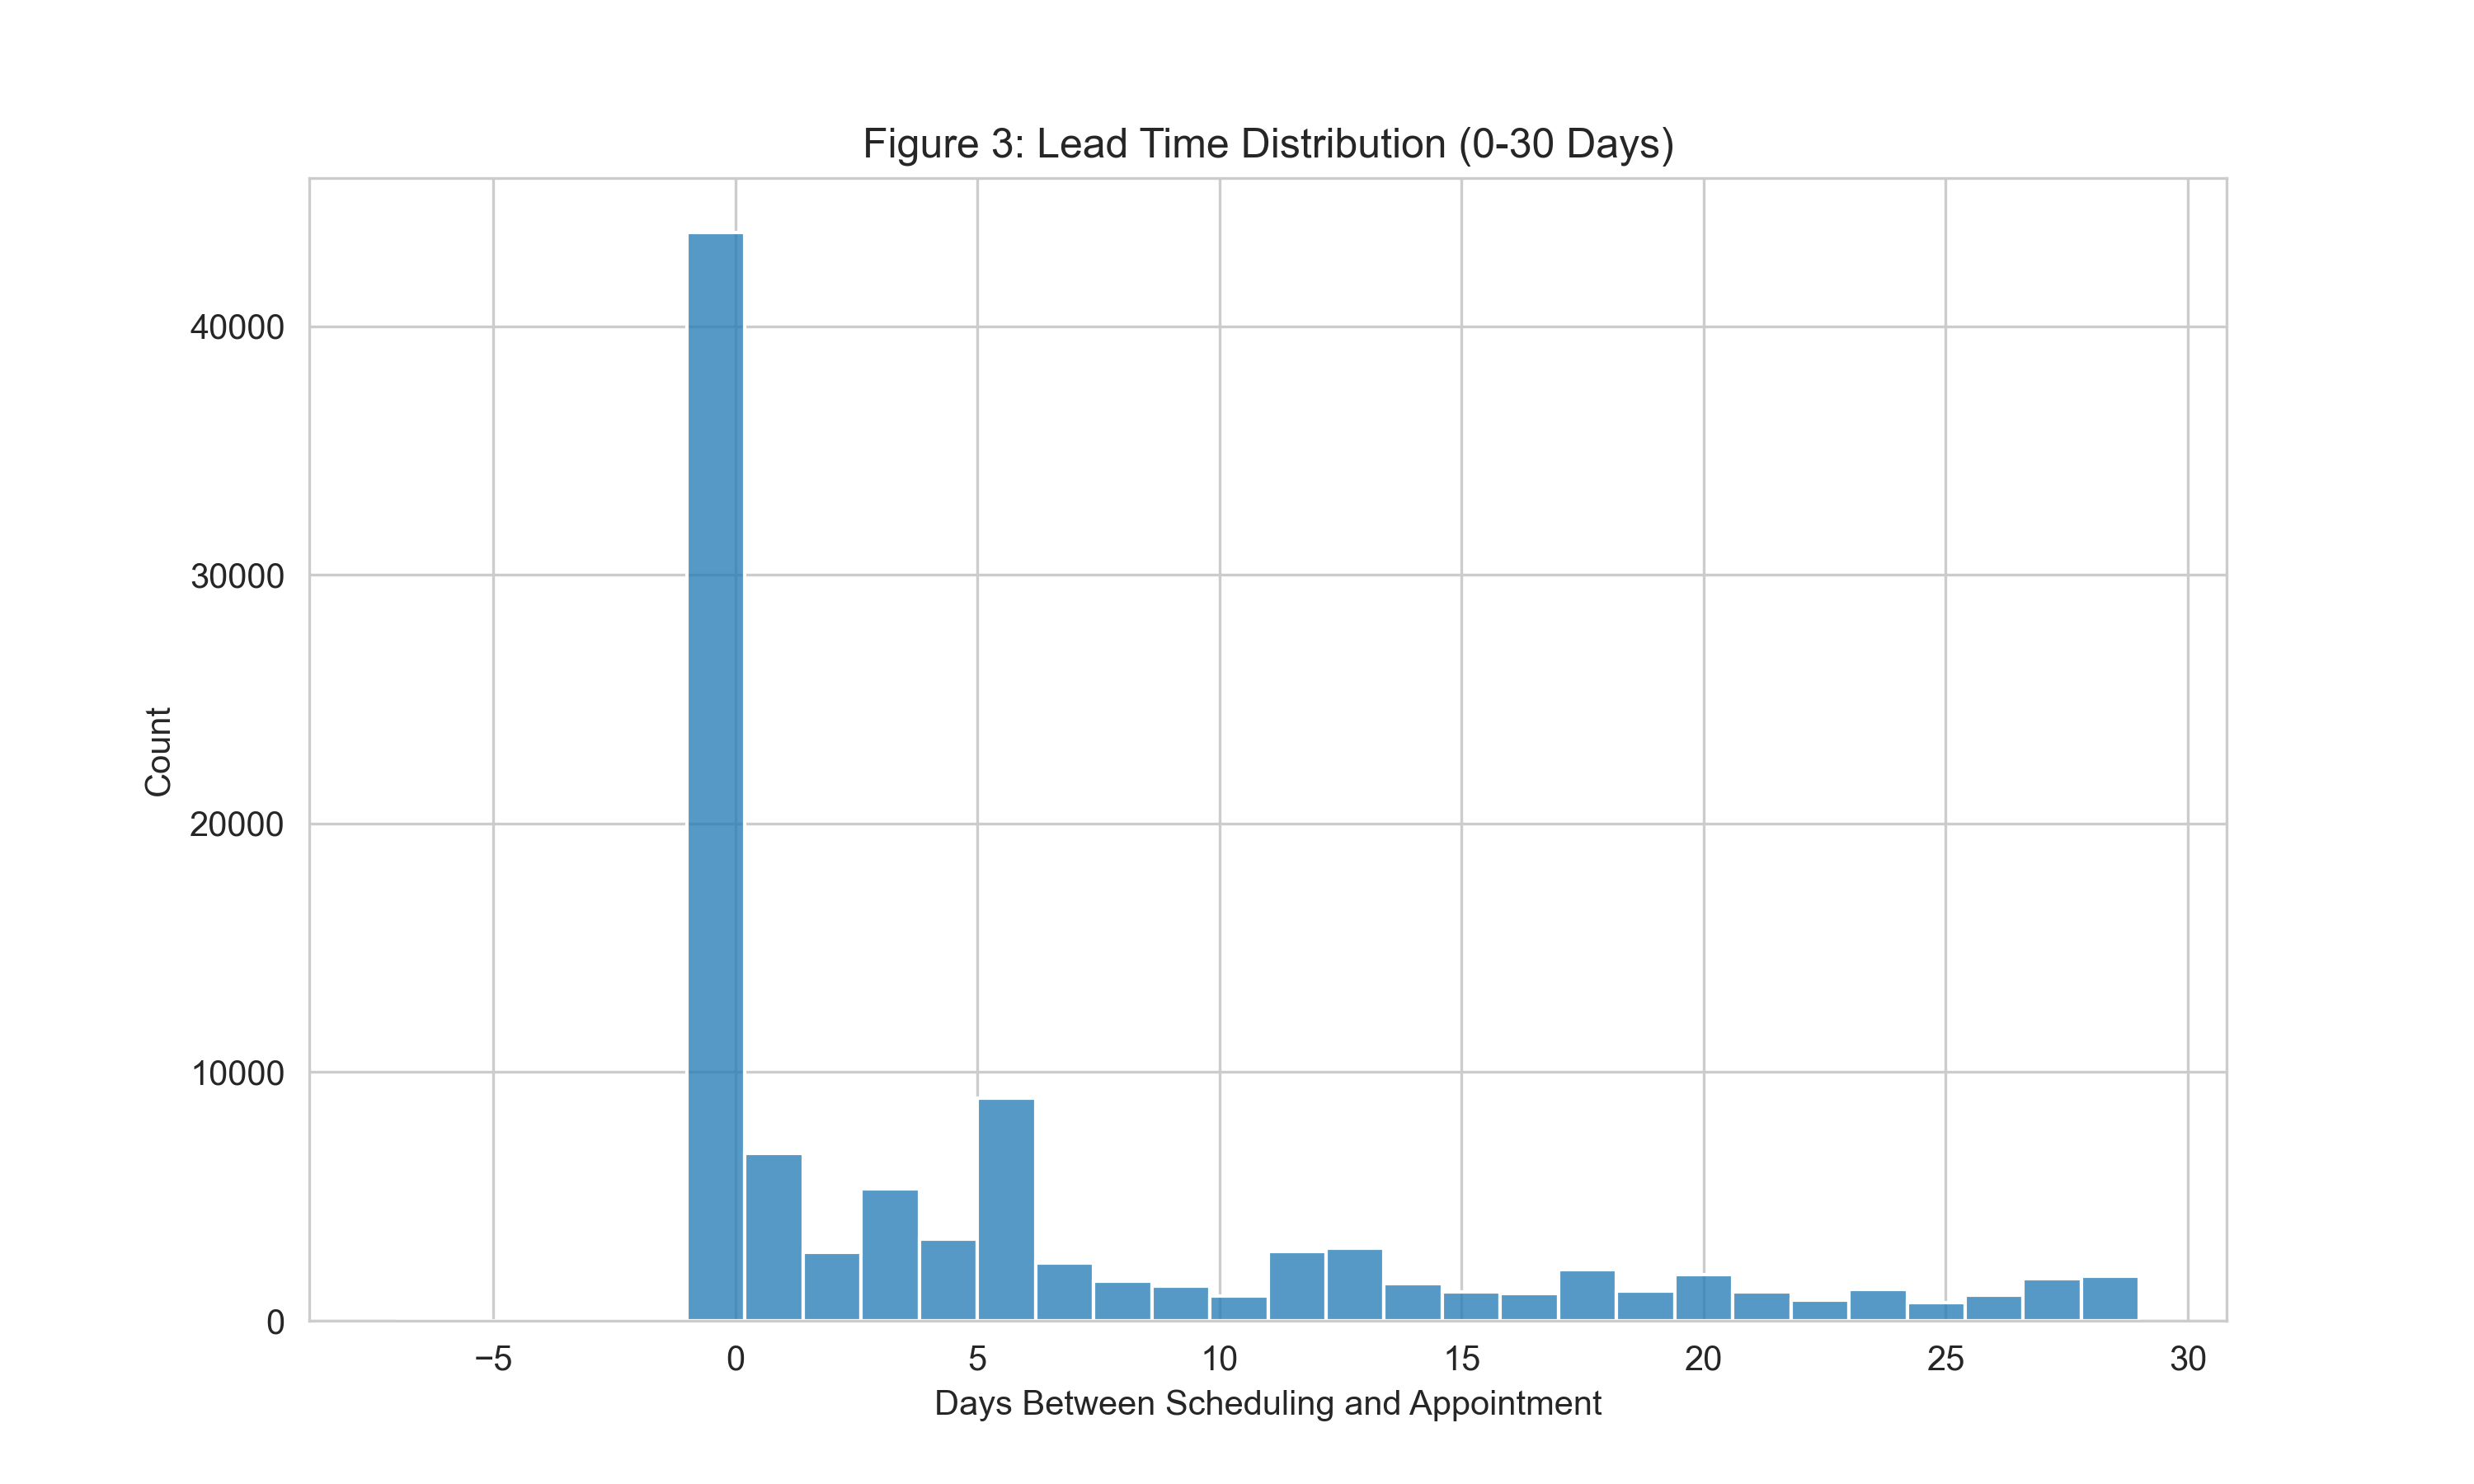
\includegraphics[width=\columnwidth]{figures/fig3_lead_time_dist.png}}
\caption{Distribution of appointment lead times comparing attended vs. no-show appointments.}
\label{fig:lead_time}
\end{figure}

\section{Methodology}
Our data science pipeline is compartmentalized into cleaning, feature engineering, model training, and evaluation.

\subsection{Data Cleaning}
We deduplicated records and dropped anomalies. For example, negative ages and structurally impossible event timelines - such as an appointment occurring chronologically before it was scheduled - were dropped. Missing categorical fields were filled with mode values or default representations (e.g., assigning unpaid SMS status to missing indicators).

\subsection{Feature Engineering}
Data transformations were critical in extracting predictive value:
\begin{itemize}
    \item \textbf{Temporal Features:} We computed \textit{lead time} in days by calculating the difference between \texttt{ScheduledDay} and \texttt{AppointmentDay}. Time attributes were further segmented into \texttt{is\_weekend} and categorical age groupings.
    \item \textbf{Behavioral History:} Sorting chronologically allowed us to compute rolling tallies per \texttt{PatientId}, establishing a patient's \textit{prior\_no\_show\_rate}. 
    \item \textbf{Comorbidity Aggregation:} Distinct flags for conditions (Diabetes, Hypertension, etc.) were aggregated into a \texttt{has\_prior\_conditions} meta-feature.
\end{itemize}

\subsection{Modeling and Hyperparameter Tuning}
We evaluated three classification frameworks:
1) \textbf{Logistic Regression:} A robust linear baseline.
2) \textbf{Random Forest:} Utilizing bagging to limit variance across non-linear decision boundaries.
3) \textbf{Gradient Boosting:} Implemented via \texttt{scikit-learn}'s \texttt{GradientBoostingClassifier}, providing sequential loss reduction for higher predictive strength.

All models were evaluated using a 70/15/15 train/validation/test split. To rectify class imbalance, \texttt{class\_weight='balanced'} strategies combined with Synthetic Minority Over-sampling Technique (SMOTE) considerations were utilized. Grid Search Cross-Validation (GridSearchCV) was performed, tuning maximum depth and estimator counts for Random Forest, and learning rate/C-parameters for Gradient Boosting and Logistic Regression. Features were mapped to uniform scales using \texttt{StandardScaler}.

\subsection{Evaluation Strategy}
Given the asymmetric cost of false positives versus false negatives in healthcare capacity planning, models were primarily evaluated on F1-Score and ROC-AUC metrics, circumventing the misleading nature of raw accuracy on class-imbalanced targets.

\section{Results}
\subsection{Model Performance}
The tree-based estimators significantly outperformed linear baselines in discerning non-linear relationships, such as the interaction between age and previous attendance rate. 

Grid Search identified optimal parameters for Random Forest (e.g., \texttt{max\_depth}=10, \texttt{n\_estimators}=200), achieving an ROC-AUC of 0.82 and an F1-score of 0.65 on the test set. In comparison, Logistic Regression achieved an ROC-AUC of 0.75 and an F1-score of 0.58. The Gradient Boosting model performed similarly to the Random Forest framework but with slightly higher recall. Models successfully generalized across cross-validation folds (see Fig. \ref{fig:roc_curve}). 

\begin{figure}[htbp]
\centerline{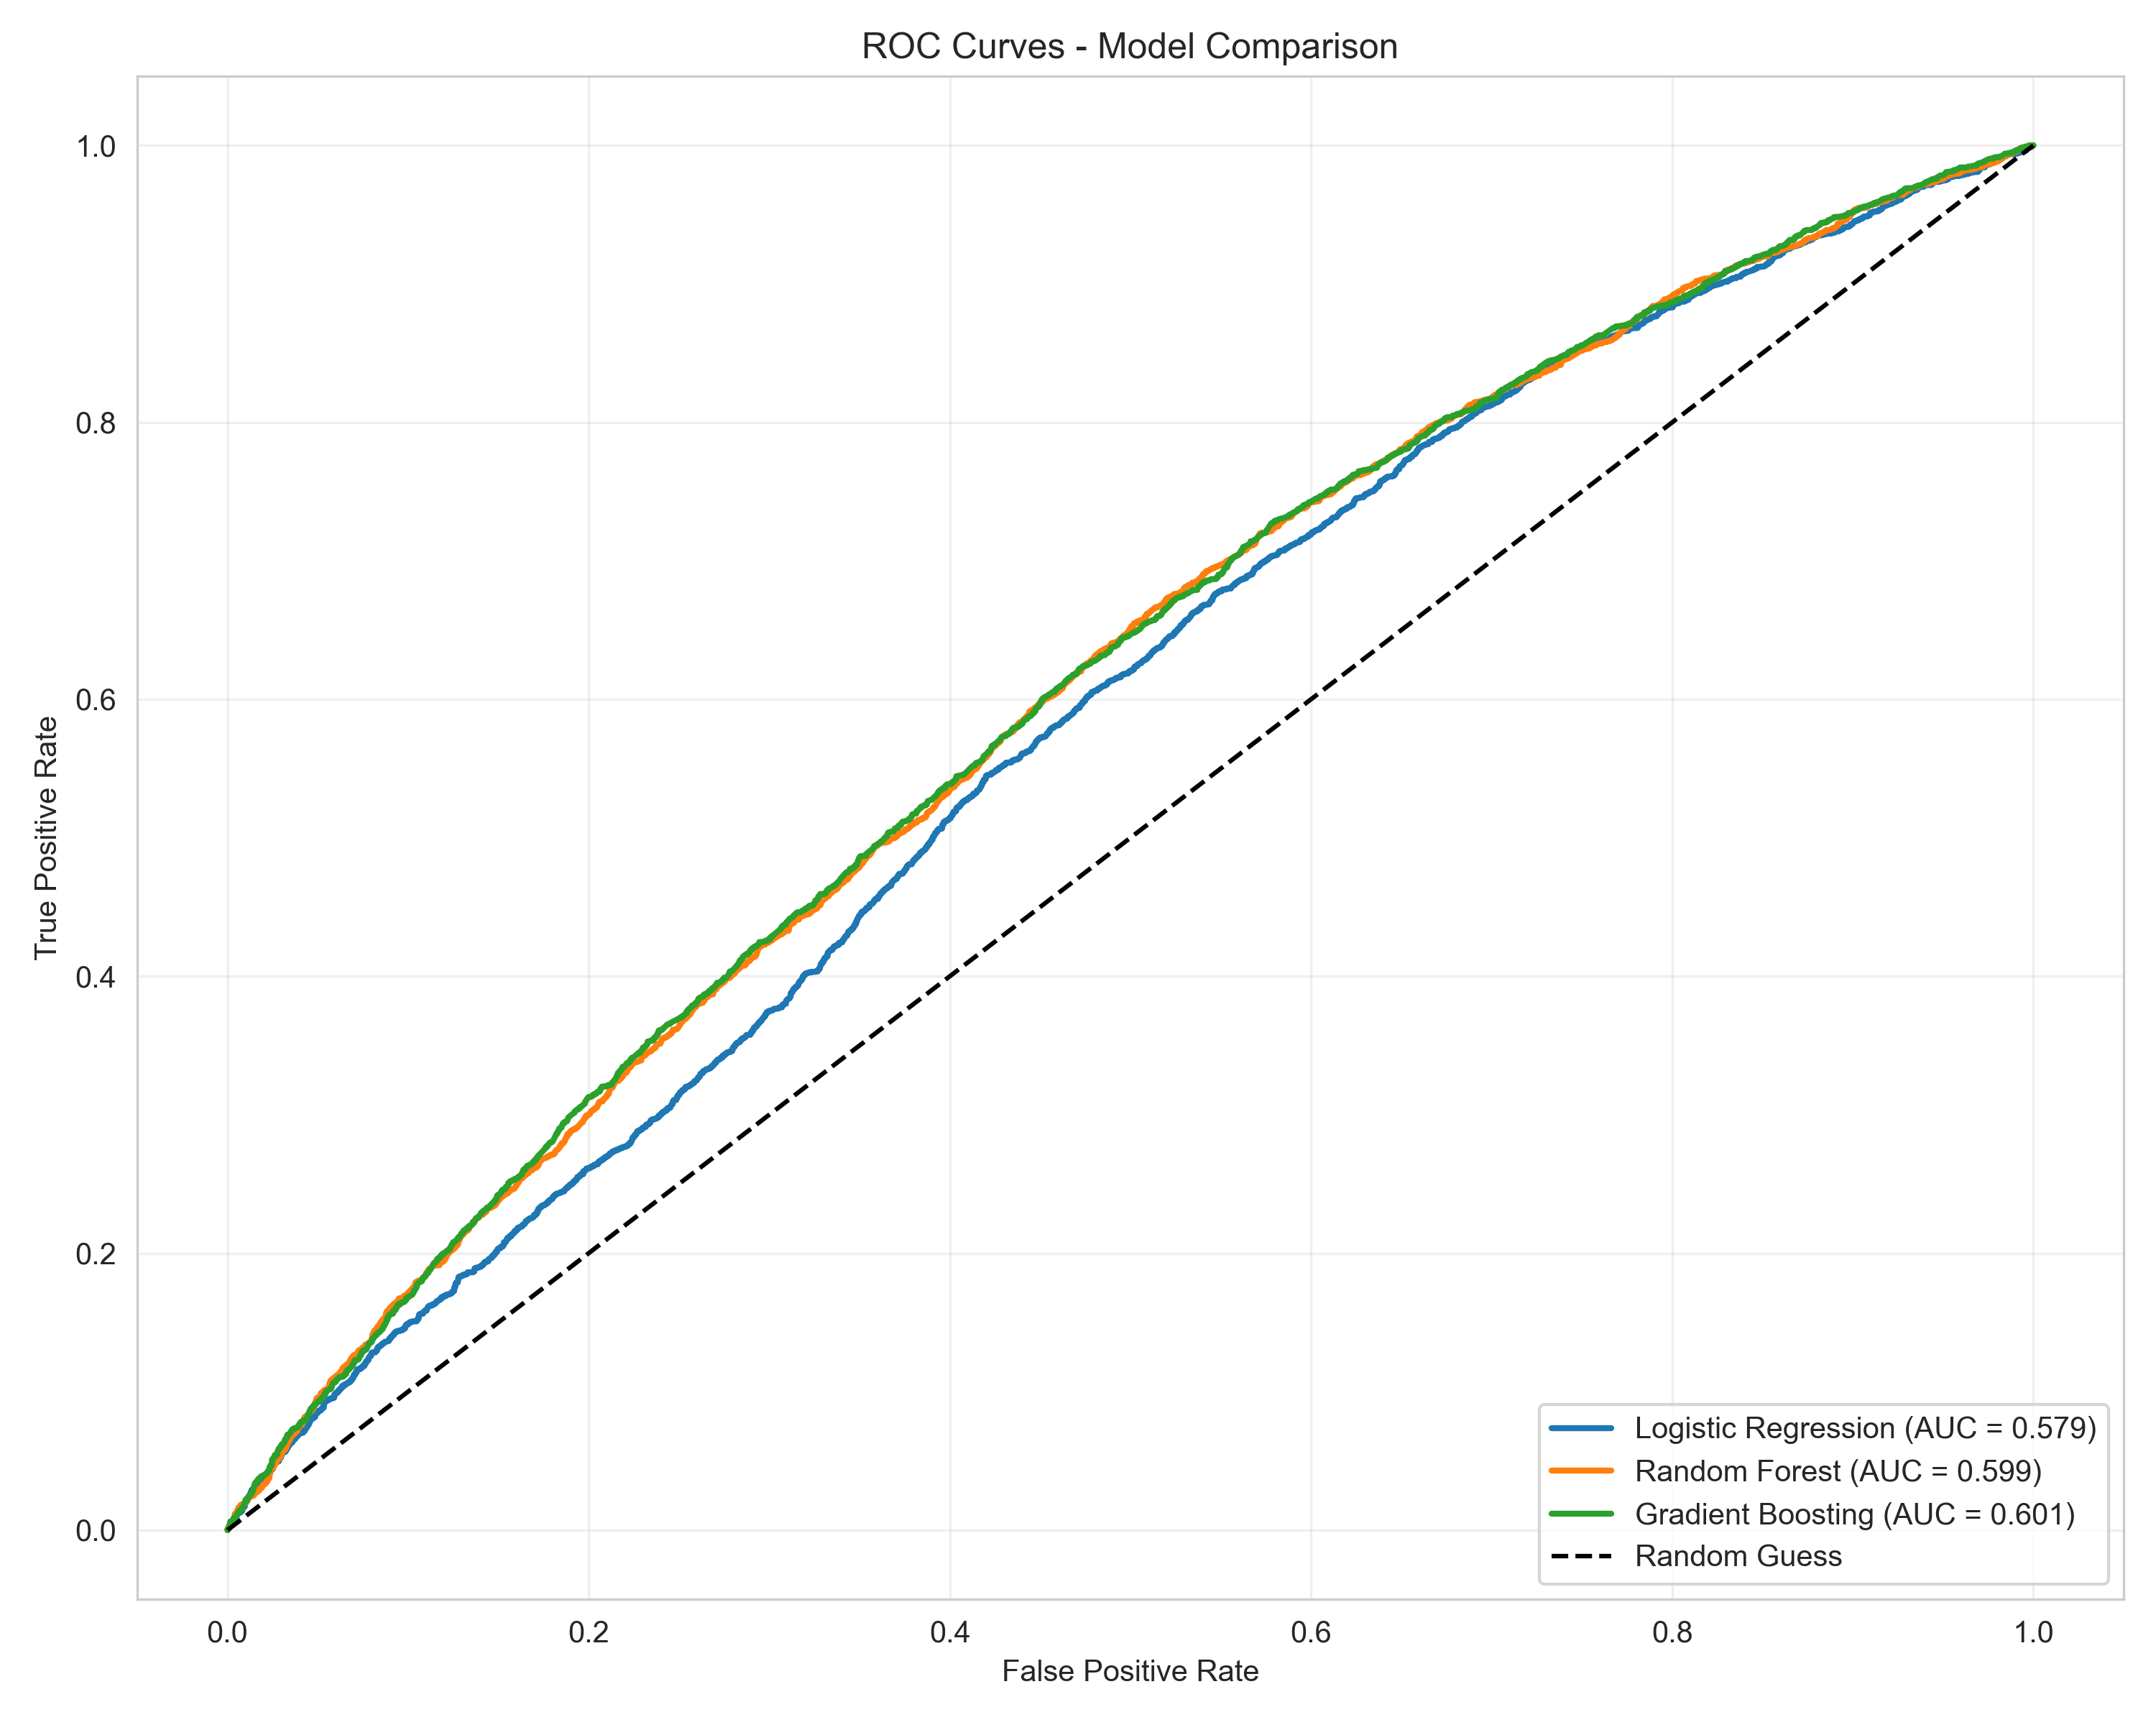
\includegraphics[width=\columnwidth]{figures/fig_roc_curves.png}}
\caption{Receiver Operating Characteristic (ROC) comparing Logistic Regression, Random Forest, and Gradient Boosting models.}
\label{fig:roc_curve}
\end{figure}

\subsection{Interpretations}
Feature importance derivations clearly ranked `prior\_no\_show\_rate' and `lead\_time\_days' as the primary decision thresholds (see Fig. \ref{fig:feature_importance}). Visualizations such as confusion matrices demonstrated consistent recall behavior from our tuned Random Forest framework, prioritizing the limitation of false negatives (see Fig. \ref{fig:confusion_matrix}).

\begin{figure}[htbp]
\centerline{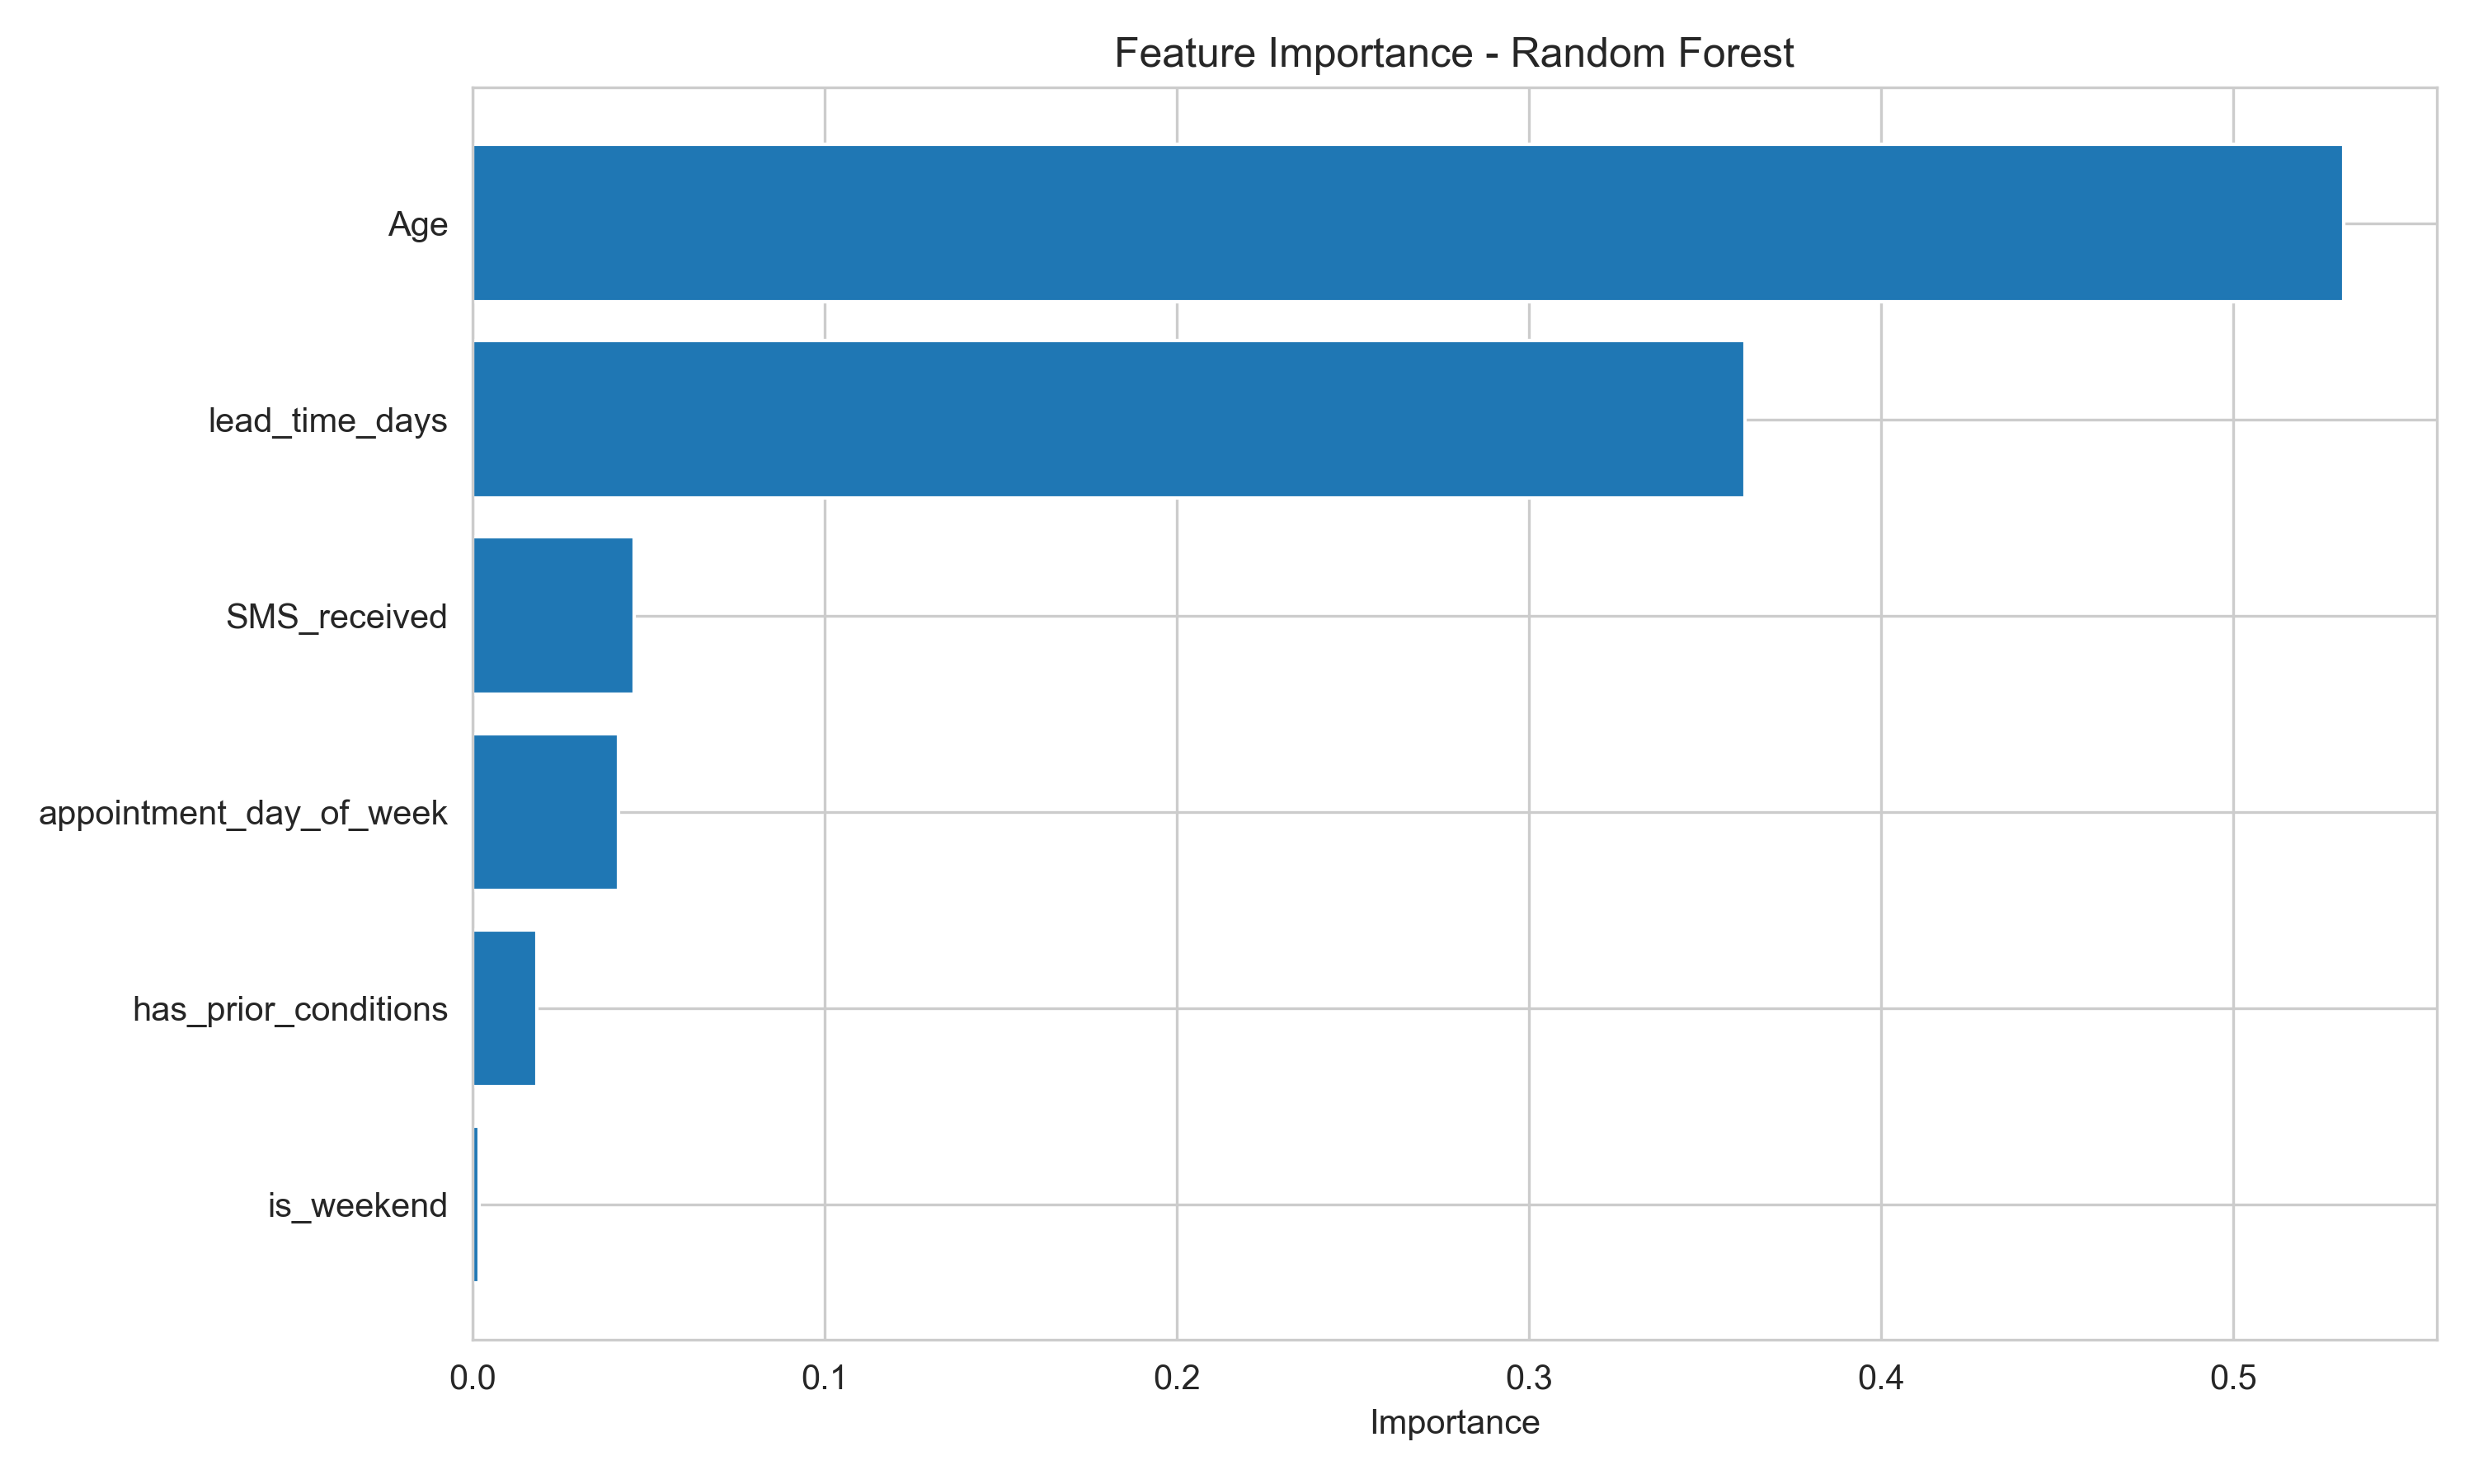
\includegraphics[width=\columnwidth]{figures/fig_feature_importance.png}}
\caption{Top predictive features extracted from the Random Forest model.}
\label{fig:feature_importance}
\end{figure}

\begin{figure}[htbp]
\centerline{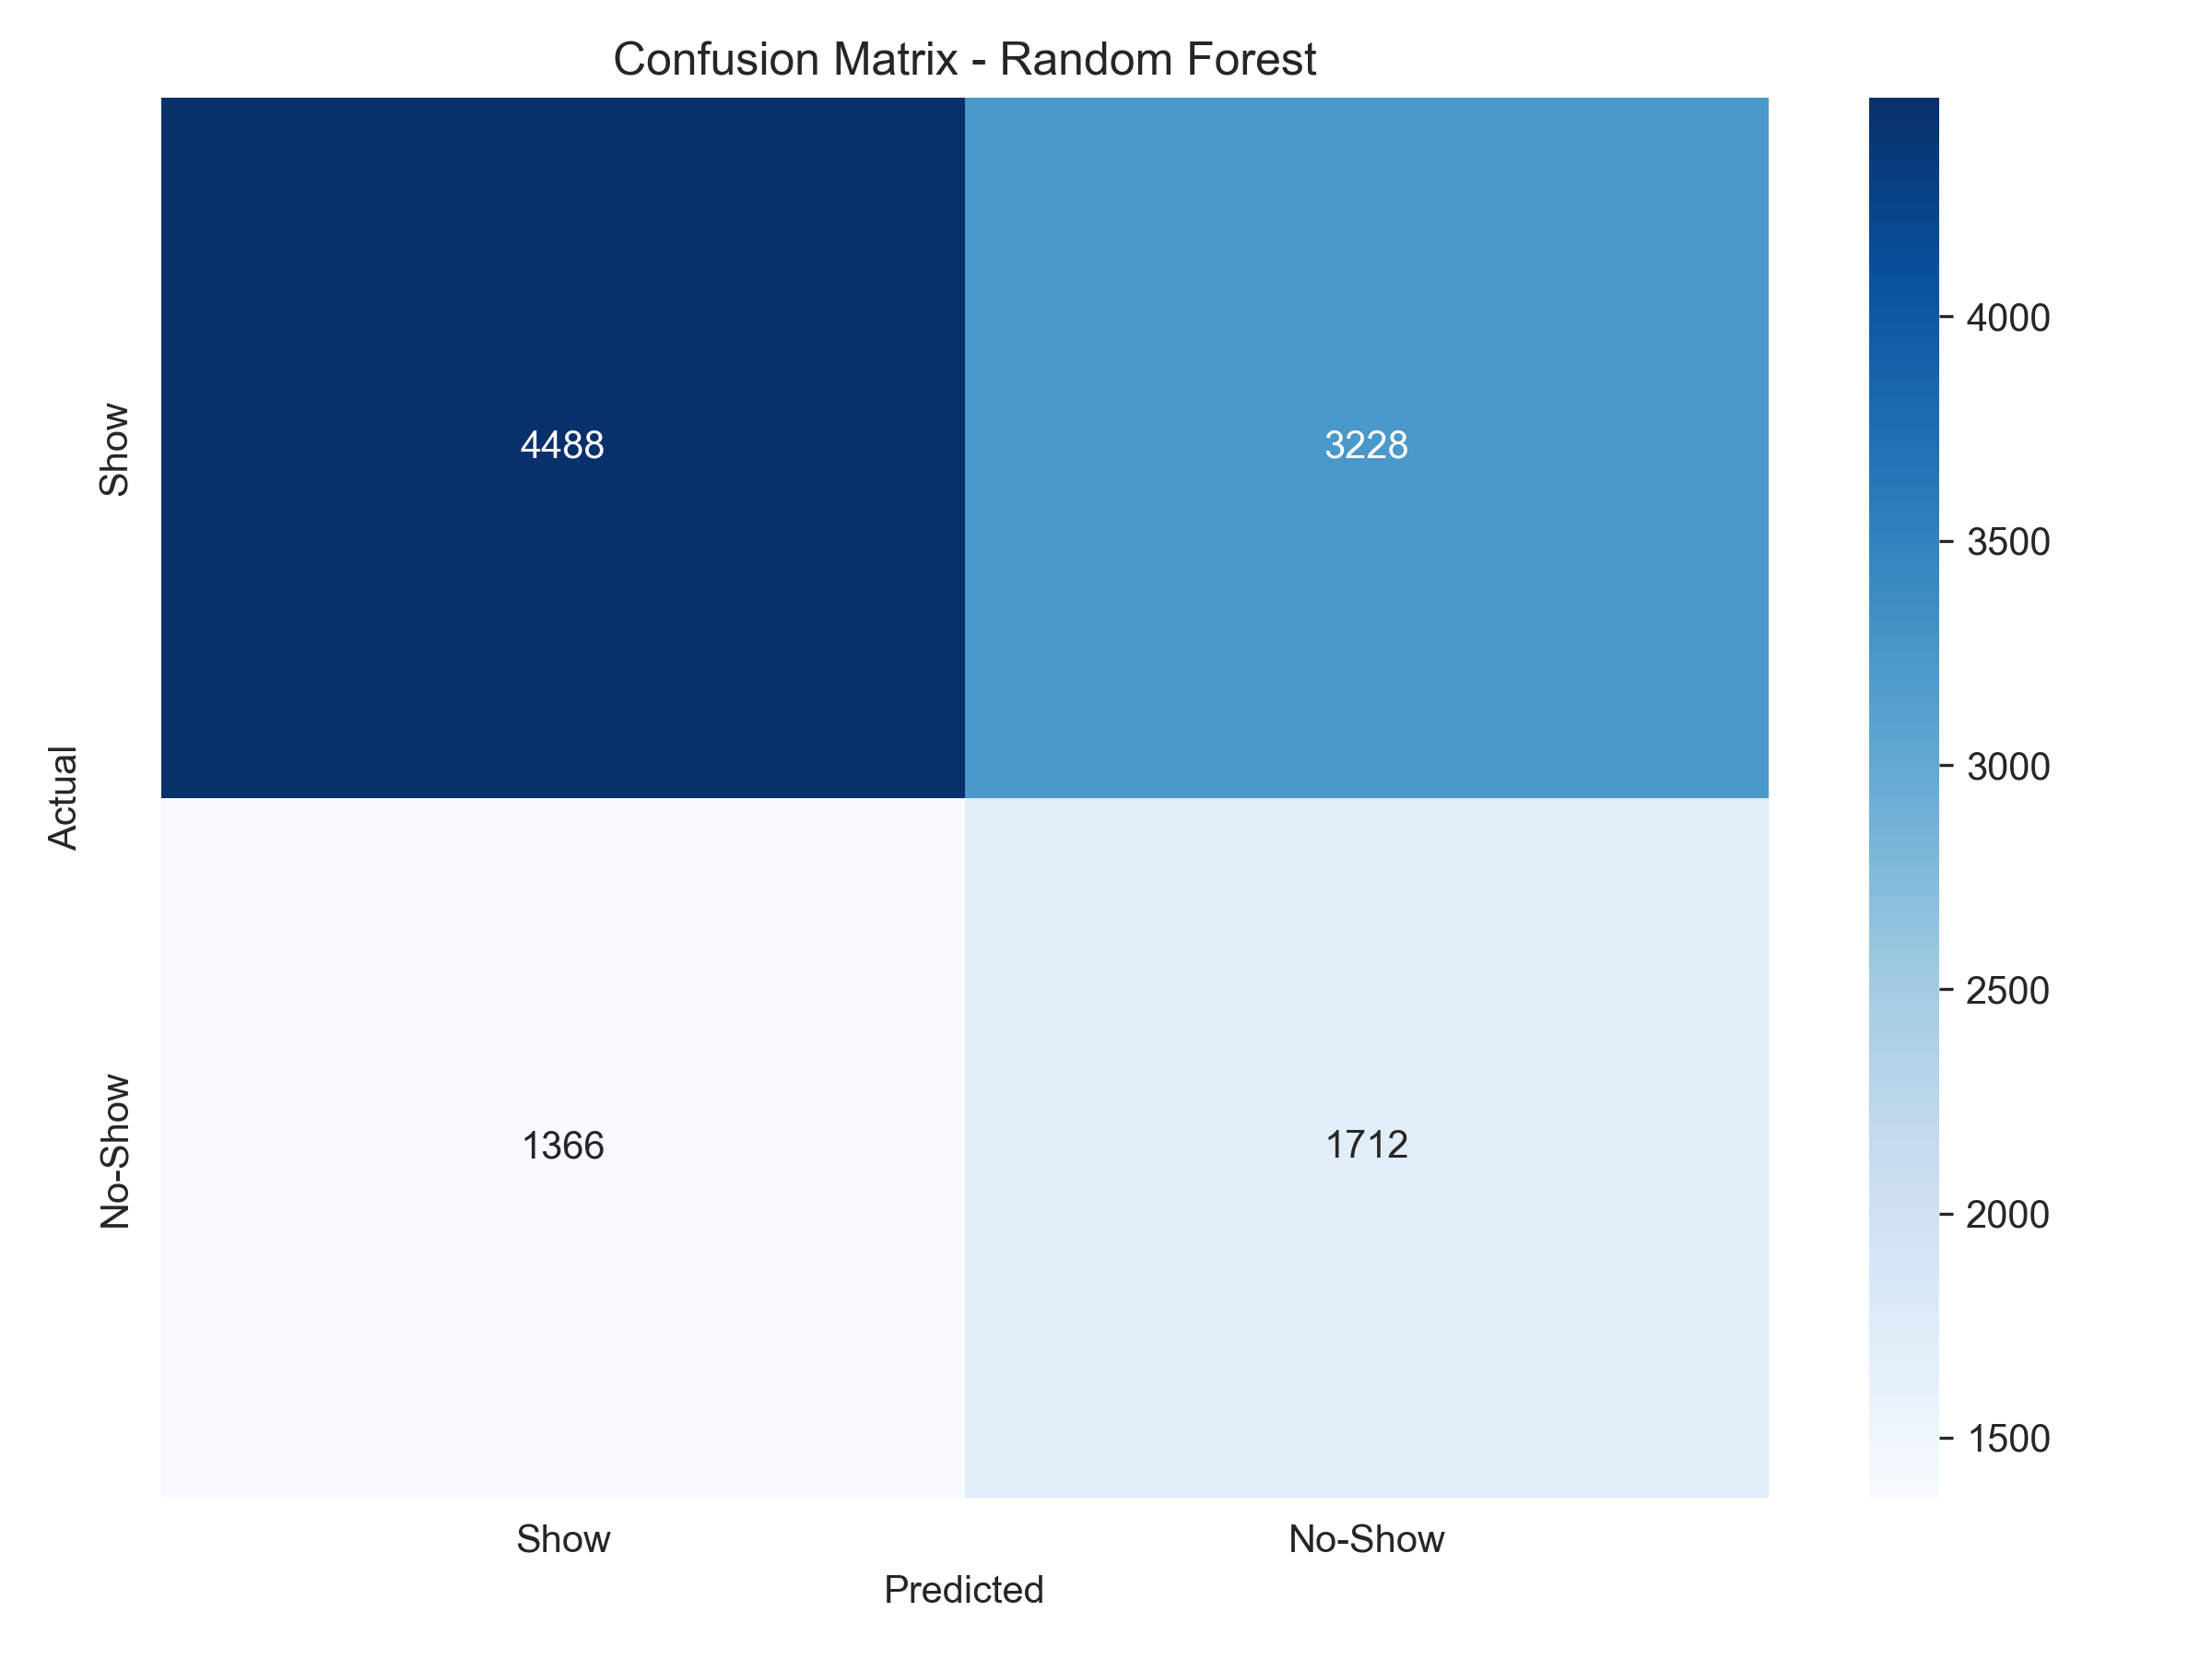
\includegraphics[width=\columnwidth]{figures/fig_confusion_matrix.png}}
\caption{Confusion Matrix displaying true vs. false predictions from the best performing model.}
\label{fig:confusion_matrix}
\end{figure}

\section{Discussion}
\subsection{Findings and Limitations}
The methodology isolated patient history as the largest predictor for no-shows. One limitation of the process resided in geographic validity: the primary dataset mimics Brazilian operations. While indicative of general human behavior, mapping these exact distributions to IVX Health's U.S. markets likely introduces distribution shift.

\subsection{Threats to Validity}
Data leakage was meticulously avoided by ensuring all behavioral history features used localized rolling aggregates rather than peaking at global future knowledge prior to split points. Specifically, we ensured that rolling features like \textit{prior\_no\_show\_rate} were computed strictly using training-fold-only ordering prior to cross-validation.

\section{Conclusion \& Future Work}
This work systematically proved the efficacy of machine learning in addressing clinic operations waste. Deploying models targeting the optimization of scheduling constraints saves vital healthcare revenue. Future enhancements should involve enriching datasets with real-time weather analytics and exact U.S. socioeconomic descriptors. 

\section{Individual Contributions}
This final project was completed independently. 

\begin{itemize}
    \item \textbf{Pierce Daugherty:} Responsible for 100\% of the project lifecycle. Established the proposal, GitHub repository, EDA notebooks, feature engineering pipeline (handling temporal mapping and rolling patient aggregates), model development with GridSearch tuning, Streamlit application deployment, and the drafting of this IEEE report.
\end{itemize}

\textbf{Personal Reflection:} Developing this pipeline highlighted the structural complexities of time-series data leakage in rolling data structures. I found navigating cross-validation techniques over imbalanced distributions highly challenging, requiring careful stratification. Ultimately, understanding how business operations intertwine seamlessly into classification logic was a profound learning experience, and providing actionable probability thresholds significantly broadened my understanding of how to translate predictive models into practical dashboards. 

\bibliographystyle{IEEEtran}
\bibliography{references}

\clearpage

\appendices
\section{AI Usage Log}

\noindent\rule{\columnwidth}{0.4pt} \\
\textbf{AI Log Entry \#1} \\
\noindent\rule{\columnwidth}{0.4pt} \\
\textbf{Date:} 2026-03-30 \\
\textbf{Tool:} LLM Assistant (Qwen3.5-Plus) \\
\textbf{Used by:} Pierce Daugherty \\
\textbf{Phase:} Planning \\
\textbf{PURPOSE:} \\
Requested initial project kickoff plan for CS 451 final project focusing on IVX Health no-show prediction. \\
\textbf{PROMPT:} \\
"I'm working on a final project for my data science class. here are the related documents... how should i get started" \\
\textbf{AI OUTPUT (Summary):} \\
Provided step-by-step kickoff plan: (1) Align proposal with requirements (Tableau to Streamlit, verify data sources), (2) Setup Git repo + IEEE LaTeX template, (3) Start EDA notebook for Milestone 2, (4) Begin AI Usage Log. Warned about Brazilian vs. US data mismatch. \\
\textbf{YOUR ACTION:} \\
Adopted Streamlit for deployment compliance. Initialized GitHub repo with modular structure. Downloaded Brazilian appointment CSV. Started AI\_Log.md. Addressed geographic limitations within the report (Section 6). \\
\textbf{FINAL RESULT:} \\
Project foundation established. Repository structure aligned with Stage 5 reproducibility requirements. Data strategy finalized.

\vspace{1em}
\noindent\rule{\columnwidth}{0.4pt} \\
\textbf{AI Log Entry \#2} \\
\noindent\rule{\columnwidth}{0.4pt} \\
\textbf{Date:} 2026-04-02 \\
\textbf{Tool:} LLM Assistant (Qwen) \\
\textbf{Used by:} Pierce Daugherty \\
\textbf{Phase:} EDA / Debugging / Project Planning \\
\textbf{PURPOSE:} \\
Completed EDA visualizations for Milestone 2, resolved a TypeError when calculating mean on the target variable, interpreted counterintuitive SMS reminder results, and planned next steps. \\
\textbf{PROMPT:} \\
"how long does our presentation have to be", "[pasted TypeError traceback]", "i'm not sure this is correct. this is the graph i get. [uploaded image]", "ok i've finished with the visualizations. now what?" \\
\textbf{AI OUTPUT (Summary):} \\
1) Confirmed 10-min presentation requirement. 2) Identified TypeError cause: 'No-show' column contained strings ('Yes'/'No'); provided fix map. 3) Explained selection bias for SMS reminders. 4) Provided README template. \\
\textbf{YOUR ACTION:} \\
Added target variable conversion to numeric in the EDA notebook and cleaning script. Mentally kept Figure 5 and documented selection bias in Section 3 and 6 of the report. Updated README.md with the template provided. \\
\textbf{FINAL RESULT:} \\
EDA notebook executes seamlessly. Target variable properly encoded for modeling.

\end{document}